\section{Introduction}%
\label{sec:ch2_intro}

Completeness as a metric has traditionally been defined under the assumption
that the photometric constraint is a flat, limiting $\Delta\textrm{mag}$ called
$\Delta\textrm{mag}_0$ \citep{brownSingleVisitPhotometric2005}, an assumption
that was used in \Cref{cha:first_paper}. This allows for fast computation of
completeness and therefore the impact of different $\Delta\textrm{mag}_0$
values on mission yield can be assessed quickly. However, when a mission's optical
system model is more established we can calculate $\Delta\textrm{mag}_0$ for
different observing scenarios, a specific combination of target, instrument,
and integration time. With more accurate $\Delta\textrm{mag}_0$ values we get a
more accurate photometric constraint and an improved value of completeness.
Ultimately, this can be used to determine which targets are worth extra
integration time.

Many factors ultimately play a role in the $\Delta\textrm{mag}_0$ for different
observing scenarios. A number of papers have described the impact of
integration time on completeness by assuming a constant $\Delta\textrm{mag}_0$
for a given integration time.\citep{hunyadiSingleVisitCompleteness2005,
brownNewCompletenessMethods2010, starkMaximizingExoEarthCandidate2014,
keithlyOptimalScheduling2020}. The $\Delta\textrm{mag}_0$ values have been
found by defining an equation for required integration time to reach a desired
signal-to-noise ratio (SNR) and inverting that equation to isolate the
$\Delta\textrm{mag}$ as a function of the integration time.
\citet{keithlyOptimalScheduling2020}, which analyzed an optical system based on
the Roman Space Telescope's coronagraph instrument \citep{Nemati2014}, used the
integration time equation,
\begin{equation}
  t = \frac{\textrm{SNR}^2 r_n}{r^2_\textrm{pl} - \textrm{SNR}^2 r^2_{\Delta I}}.
  \label{eq:2020t}
\end{equation}
which has been used for a number of exoplanet direct imaging studies
\citep{nematiSensitivityWFIRST2017, delacroixScienceYield2016,
savranskyMultimissionModeling2017}, and expand the planet count rate term,
$r_\textrm{pl}$, in terms of $\Delta\textrm{mag}$ to find the following
equation
\begin{equation}
  \Delta\textrm{mag}_i(t_{\textrm{int},i}) = -2.5 \log_{10} \frac{\textrm{SNR} \sqrt{\frac{r_{n,i}
    }{t_i} + r^2_{\Delta I, i} }}{C_{\mathcal{F}_0} 10^{-0.4 \nu_i (\lambda)}
T(\lambda, \alpha) \epsilon_{\textrm{PC}}}
  \label{eq:dean_dmag}
\end{equation}
where $t_{\textrm{int},i}$ is the integration time of the $i$'th target,
$r_{n,i}$ is the random variance count rate (or background noise count rate),
$r_{\Delta I,i}$ is the residual speckle count rate (the count rate of speckle noise after post processing effects),
$C_{\mathcal{F}_0}$ is the spectral flux density,
$\lambda$ is the observing wavelength,
$\nu_i$ is the target star's apparent magnitude,
$\alpha$ is angular separation between the planet and its star,
$T$ is the instrument's core throughput (the fraction of the planet's light collected by
the primary that ends up inside the area circumscribed by the half-max contour
of the planet's PSF \citep{Nemati2020a}), and $\epsilon_{\textrm{PC}}$ is the
photon-counting efficiency of the system.

\citet{keithlyOptimalScheduling2020} notes that $T$ is a function of $\alpha$,
but that without assuming a constant $\alpha$ the calculation of completeness
becomes much slower, as the limiting $\Delta\textrm{mag}$ becomes a function of
$\alpha$, and that the completeness values may be inaccurate for instruments
where core throughput changes considerably with $\alpha$. In this work, we
describe how to calculate the $\Delta\textrm{mag}_0$ when the
$C_{\textrm{b},i}$ term is coupled to the planet count rate $C_{\textrm{p},i}$.
In \Cref{sec:Coupling of background and planet signal} we describe a problem
that arises from an optical system model where the planet signal and the
background signal are coupled, then in \Cref{sec:numerically_inverting_ETC} we
show a numerical method for solving the signal coupling problem. In
\Cref{sec:coupling_results} we describe how to use the numerical method to
calculate accurate completeness values for known planets for the various Roman
Space Telescope's coronagraph instrument (Roman CGI) observing scenarios.
Ultimately we show the ten highest completeness planets for the Roman CGI.

\section{Coupling of background and planet signal} % (fold)
\label{sec:Coupling of background and planet signal}

The optical system laid out in \citet{keithlyOptimalScheduling2020} to create
\Cref{eq:dean_dmag}, based on the work of Bijan Nemati for the Roman CGI
\citep{Nemati2014, nematiSensitivityWFIRST2017, Nemati2020a}, works on the
assumption that the noise sources included in $C_{\textrm{b}}$ have no
dependence on the planet's $\Delta\textrm{mag}$. However, in newer formulations
of the Roman CGI exposure time calculator (ETC), there is such a dependence. Every
frame results in readout and clock-induced charge noise, and a brighter signal
will require a shorter exposure time per frame, resulting in more total frames
and therefore more total readout and clock-induced charge noise. The newer form
of the ETC is implemented in the \code{EXOSIMS} package's \code{Nemati\_2019}
module \citep{savranskyWFIRSTAFTACoronagraphScience2015} which is an adaptation
of the Roman CGI team's internal ETC.

\begin{figure}
  \begin{center}
    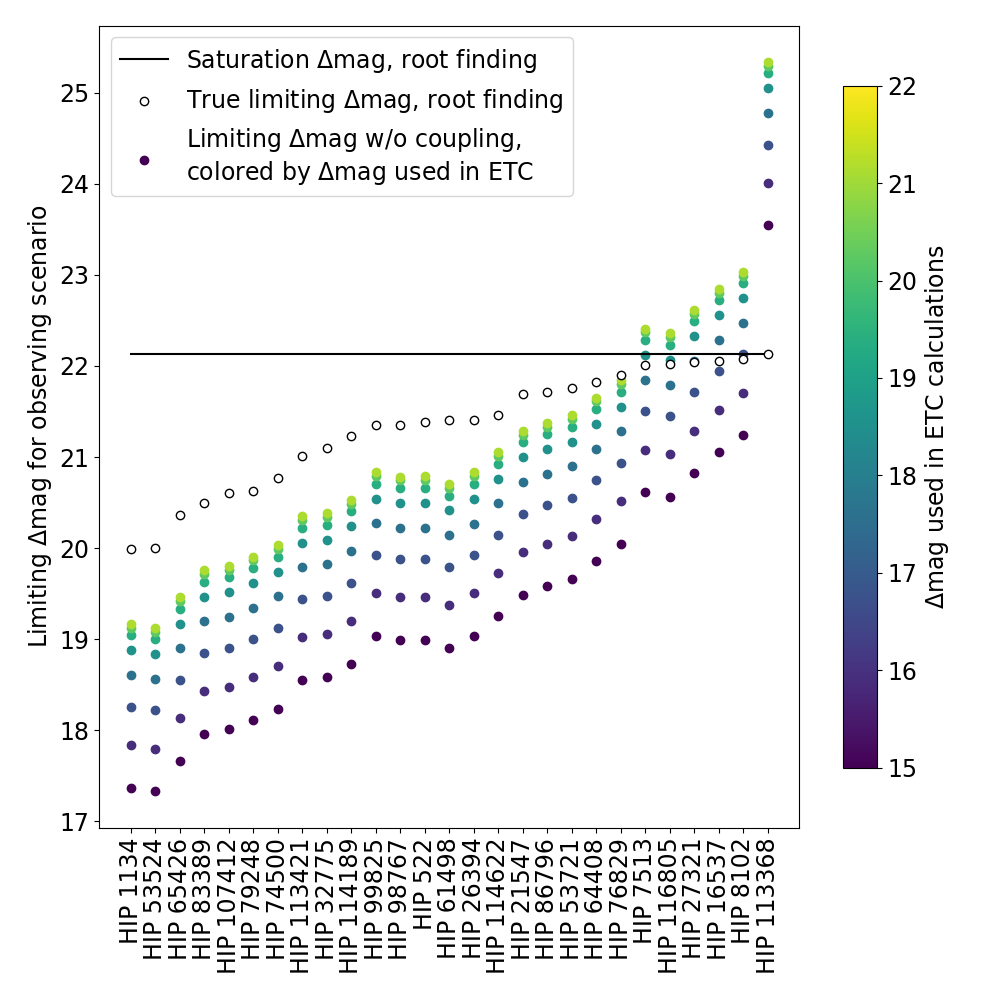
\includegraphics[width=0.95\textwidth]{ch2/figures/coupling.png}
  \end{center}
  \caption{Demonstrating the errors in limiting $\Delta\textrm{mag}$, the
  photometric constraint for completeness, when not treating the coupling
  between the planet signal and the noise factors. The observing scenario
  used for this plot is one day of integration time, the ``OPTI\_NF\_Imager''
  observing mode from the Roman CGI ETC, the target planet is fixed to an
  angular separation of $0.2955$ arcsec, zodiacal light surface brightness is fixed to
  $23 (\textrm{mag}/\textrm{arcsec})^2$, and exozodiacal light surface brightness is
  fixed to $22 (\textrm{mag}/\textrm{arcsec})^2$. The target stars included are the defaults
  in the Roman CGI ETC.}
  \label{fig:CGI_coupling}
\end{figure}

\begin{figure}
  \begin{center}
    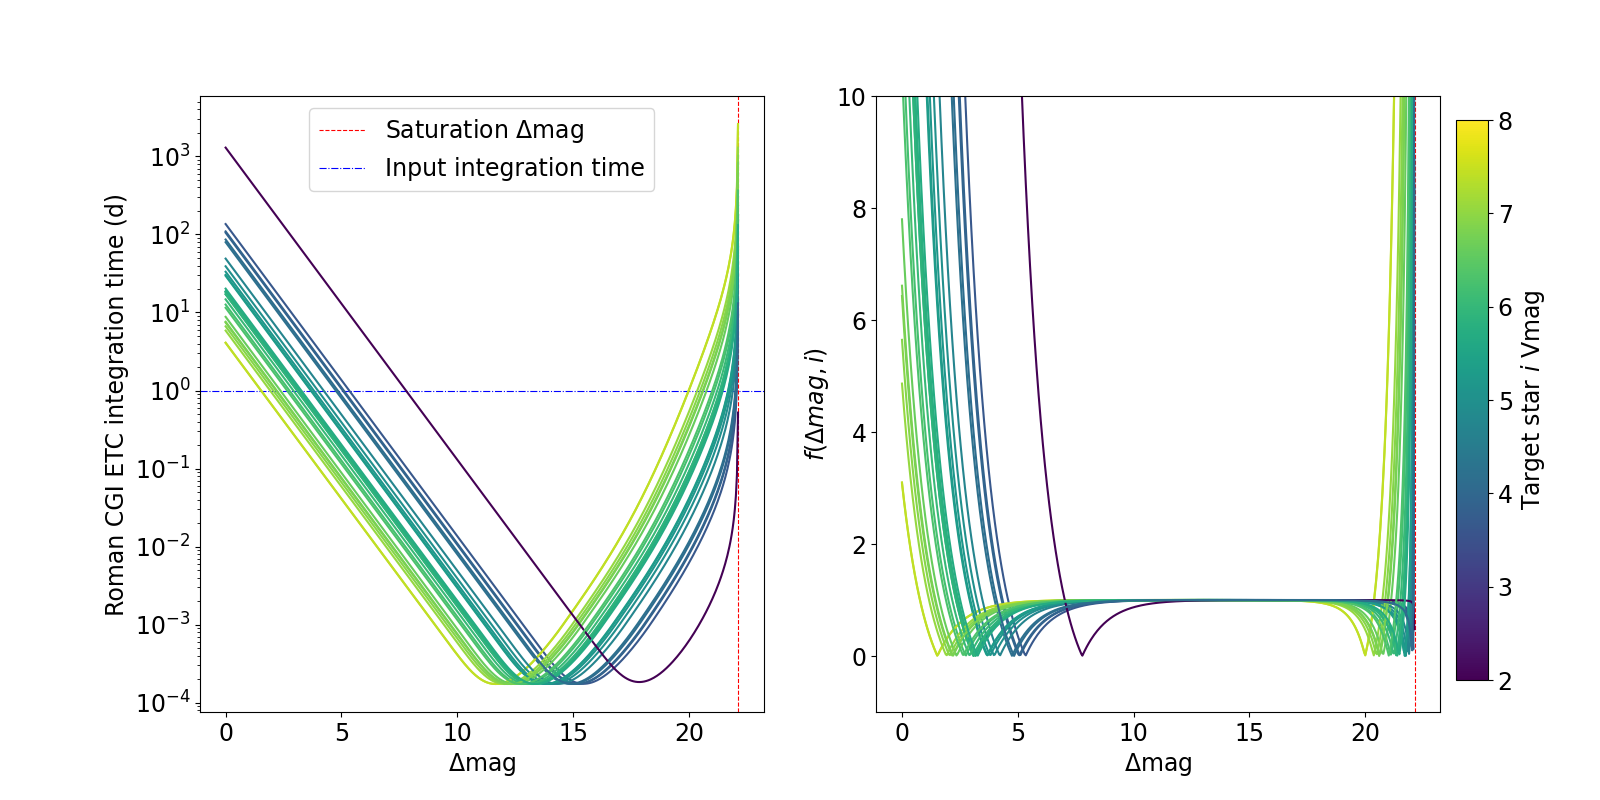
\includegraphics[width=0.95\textwidth]{ch2/figures/ETC_dMag_function.png}
  \end{center}
  \caption{Showing the Roman CGI's ETC integration time response to varying
  $\Delta\textrm{mag}$. Astrophysical inputs here are the same
  as in \Cref{fig:CGI_coupling}.}
  \label{fig:ETC_dMag_function}
\end{figure}

% \section{Coupling rewrite} % (fold)
% \label{sec:Coupling rewrite}
% STANDARDIZE TO ALL OF NEMATI 2020
The equation of signal-to-noise to noise ratio for the Roman CGI is modeled as
\begin{equation}
  \textrm{SNR} = \frac{r_\textrm{pl}t}{\sqrt{r_n t + r^2_{\Delta I} t^2}}
  \label{eq:2020SNR}
\end{equation}
% where SNR is the signal-to-noise ratio, $r_\textrm{pl}$ is the planet count
% rate, $t$ is the integration time, $r_n$ is the random variance count rate
% (background), and $r_{\Delta I}$ is the residual speckle rate, or the count
% rate of speckle noise after post processing effects. 
To calculate an exposure time for a specific SNR, planet, and star we can keep
the SNR, $r_\textrm{pl}$, $r_n$, and $r_{\Delta I}$ values constant and solve
for $t$ to get \Cref{eq:2020t}.
% \begin{equation}
%   t = \frac{\textrm{SNR}^2 r_n}{r^2_\textrm{pl} - \textrm{SNR}^2 r^2_{\Delta I}}.
%   \label{eq:2020t}
% \end{equation}
In a similar manner to calculating the
exposure time, the limiting $r_\textrm{pl}$ has traditionally been calculated
by solving \Cref{eq:2020SNR} as
\begin{equation}
  r_\textrm{pl} = \frac{\textrm{SNR} \sqrt{r_n t + r^2_{\Delta I} t^2}}{t}
  \label{eq:2020rpl}
\end{equation}
which is a useful quantity because it is the lowest planet count rate that meets
the required SNR. If we can isolate $r_\textrm{pl}$ then we can calculate a
$\Delta\textrm{mag}$ because
\begin{equation}
  r_\textrm{pl} = F_\lambda \Delta \lambda 10^{-0.4 \Delta \textrm{mag}} A \tau_\textrm{pl} \eta
  \label{eq:2020rpl_expand}
\end{equation}
where $F_\lambda$ is the spectral flux, $\Delta \lambda$ is the filter
bandwidth, $A$ is the collecting area, $\tau_\textrm{pl}$ is the throughput for
the planet light, and $\eta$ is the detector quantum efficiency. If we have a
specific $r_\textrm{pl}$ that represents the lowest possible value that reaches
the required SNR, then solving \Cref{eq:2020rpl_expand} for
$\Delta\textrm{mag}$ represents $\Delta\textrm{mag}_0$.

The trouble arises from the fact that in the newer formulation of the optical
system the $r_n$ term is now dependent on $r_\textrm{pl}$ in a significant
fashion. The equation is
\begin{equation}
  r_n = r_\textrm{pl} + k_\textrm{sp} r_\textrm{sp} + k_\textrm{lz}
  r_\textrm{lz}+ k_\textrm{ez} r_\textrm{ez}+ k_\textrm{det} r_\textrm{det}.
  \label{eq:rn}
\end{equation}
In \Cref{eq:rn} $r_\textrm{sp}$ is the speckle count rate, $r_\textrm{lz}$ is the count
rate of local zodiacal light, $r_\textrm{ez}$ is the count rate of
exozodical light, $r_\textrm{det}$ is the count rate of detector noise, and the
$k_x$ terms are variance enhancement factors for each count rate to account for
the effects of reference differential imaging. This has a clear dependence on
$r_\textrm{pl}$ but it has a further dependence through the $r_\textrm{det}$ term
in
\begin{equation}
  r_\textrm{det} =  m_\textrm{pix}\left( i_d +
  \frac{q_\textrm{CIC}}{t_\textrm{fr}} +
\frac{\sigma^2_\textrm{rd}}{t_\textrm{fr} G_\textrm{EM}} \right)
  \label{eq:rdet}
\end{equation}
where $i_d$ is the detector dark current, $m_{\textrm{pix}}$ is the number of
detector pixels that the planet signal covers, $q_{\textrm{CIC}}$ is the CCD
clock-induced charge, $t_{\textrm{fr}}$ is the frame duration,
$\sigma_{\textrm{rd}}$ is read noise, and $G_{\textrm{EM}}$ is the electron
multiplication gain. $\sigma_{\textrm{det}}^2$ is one of the four random noise
components for the target star in $C_{\textrm{b},i}$ (see \citet{Nemati2020a}
for more details). The $1/t_{\textrm{fr}}$ terms in
\Cref{eq:rdet} represent that the $q_\textrm{CIC}$
and $\sigma_\textrm{rd}$ terms are dependent on how many frames are taken over
the course of an observation. The equation for $t_\textrm{fr}$ is 
\begin{equation}
  t_{\textrm{fr}} = \frac{0.1}{DC +\left(r_{\textrm{pl}}+r_{\textrm{lz}}+r_{\textrm{ez}}+r_{\textrm{sp}}\right)/m_{\textrm{pix}}}
  \label{eq:bijan_frame_duration}
\end{equation}
where $DC$ is the detector dark current noise per second.
\Cref{eq:bijan_frame_duration} comes from the Roman CGI team and is restricted
to be between 1 and 80 seconds (personal communication, Oct 5, 2022).

To complicate the relationship further, the $t_{\textrm{fr}}$ value impacts the
number of cosmic ray hits per frame and the charge transfer efficiency. Those
end up impacting the detector degradation which then impacts all count
rates. 
By making $r_n$ a complex function of $r_\textrm{pl}$ we are unable to isolate
it as a function of SNR, $r_n$, $r_{\Delta I}$, and $t$ analytically. Therefore
to calculate the $\Delta\textrm{mag}_0$ for a specific observing scenario we
need to invert the relationship numerically.

\Cref{fig:CGI_coupling} shows the errors that occur when trying to
calculate the $\Delta\textrm{mag}_0$ values without accounting for the rate
coupling. The colored circles represent calculating $\Delta\textrm{mag}$
from \Cref{eq:2020rpl,eq:2020rpl_expand} and using a constant
$\Delta\textrm{mag}$ value for the $r_n$ term. The true $\Delta\textrm{mag}$
values, the empty circles, deviate significantly and in many cases would result
in underestimating $\Delta\textrm{mag}_0$. The direction of the error is driven
by how close the $\Delta\textrm{mag}_0$ is to the saturation
$\Delta\textrm{mag}$, or the $\Delta\textrm{mag}$ at which $\left(\textrm{SNR}
\cdot r_{\Delta I}\right)^2$ becomes greater than $r_{\textrm{pl}}$ in
\Cref{eq:2020t} and the calculated integration times become
negative.

% section sec:Coupling rewrite (end)


\section{Numerically Inverting the Roman CGI Exposure Time Calculator}
\label{sec:numerically_inverting_ETC}

To restate the problem, we want to determine the completeness for a given
integration time, $t_{\textrm{int}}$. The photometric constraint in the
completeness calculation is defined as the dimmest planet that meets the
required SNR. However, the brightness of that planet affects both the signal
and the noise. Failing to account for the changes in the noise term can lead to
overly optimistic photometric constraints, systematically over estimating
completeness. By inputting different $\Delta\textrm{mag}$ values in the
ETC, with the SNR fixed to the required value, we can
determine which $\Delta\textrm{mag}$ results in the integration time
$t_{\textrm{int}}$ that we are trying to calculate completeness for.

Repeatedly running the ETC is computationally costly so we formulate it as a
minimization problem to reduce the number of evaluations necessary. The
objective function for this minimization is
\begin{equation}
  f(\Delta\textrm{mag}, i) = |t_{\textrm{int}} -
  t_{\textrm{ETC}}(\Delta\textrm{mag}, \textrm{SNR}, i)|
  \label{eq:intTime_root_obj}
\end{equation}
where $t_{\textrm{ETC}}$ is a call to our ETC for target star $i$ for a
specific observing scenario. The minimization is complicated by the fact that
$f\left(\Delta\textrm{mag}, i\right)$ has two minima, as shown on the right plot of
\Cref{fig:ETC_dMag_function}. As we are looking for
$\Delta\textrm{mag}_0$, our goal is to converge to the larger of the local
$\Delta\textrm{mag}$ minima. The lower of the minima is caused by the model for
$C_b$ increasing exponentially as $\Delta\textrm{mag}$ goes to zero. The target
star's V magnitude affects the location where the slope changes, which can be
seen in \Cref{fig:ETC_dMag_function} where the line colors represent the V
magnitude.

The ETC also has a saturation value, $\Delta\textrm{mag}_\textrm{sat}$. At
$\Delta\textrm{mag}_\textrm{sat}$ the integration time goes to infinity,
representing the $\Delta\textrm{mag}$ where even an infinite integration time
would be insufficient to detect a planet of that $\Delta\textrm{mag}$. Any
$\Delta\textrm{mag}$ value greater than $\Delta\textrm{mag}_\textrm{sat}$ also
will never be detected. $\Delta\textrm{mag}_\textrm{sat}$ is marked as an
asymptote in \Cref{fig:ETC_dMag_function}. Because of this we will use the
$\Delta\textrm{mag}_\textrm{sat}$ as the upper bound for our minimization,
$\Delta\textrm{mag}_{ub}$. The $\Delta\textrm{mag}_{ub}$ can be found by
running root finding on 
\begin{equation}
  C_{\textrm{p}} - \left(\textrm{SNR} \cdot C_{\textrm{sp}}\right)^2
  \label{eq:sat_root}
\end{equation}
for different values of $\Delta\textrm{mag}$.

The lower bound should be set such that the domain of $f\left(\Delta\textrm{mag},
i\right)$ is limited to the $\Delta\textrm{mag}$ values where the integration
times are strictly increasing so that the minimization doesn't converge to the
lower bound because it is approaching the lower $\Delta\textrm{mag}$ minima. As
a heuristic, we begin with
\begin{equation}
  \Delta\textrm{mag}_{lb}(i) = \Delta\textrm{mag}_{ub}(i) - 2 - V(i)
  \label{eq:dMag_lb}
\end{equation}
which resulted in convergence for the minimization in over 99\% of cases for
the Roman CGI's narrow field of view imaging instrument. The routine is implemented
as the \code{calc\_dMag\_per\_intTime} function in the \code{Nemati}
module in the \code{EXOSIMS} package. The minimization function itself
is \code{SciPy}'s \citep{virtanenSciPyFundamental2020} implementation of the
bounded scalar minimization routine from \citet{forsytheComputerMethods1977}
with a tolerance of $10^{-8}$ on $f(\Delta\textrm{mag}, i)$. The function
requires as input the local and exozodiacal light surface brightnesses,
as they are required by the CGI's ETC. In this work, we use a local zodiacal
light surface brightness of $Z=23
\frac{\textrm{mag}}{\textrm{arcsec}^2}$ and exozodiacal light surface
brightness of $EZ=22 \frac{\textrm{mag}}{\textrm{arcsec}^2}$
taken from \citet{starkMaximizingExoEarthCandidate2014}. Some example
minimization calculations are shown in \Cref{fig:minimization_star_comp}.
\begin{figure}
  \begin{center}
    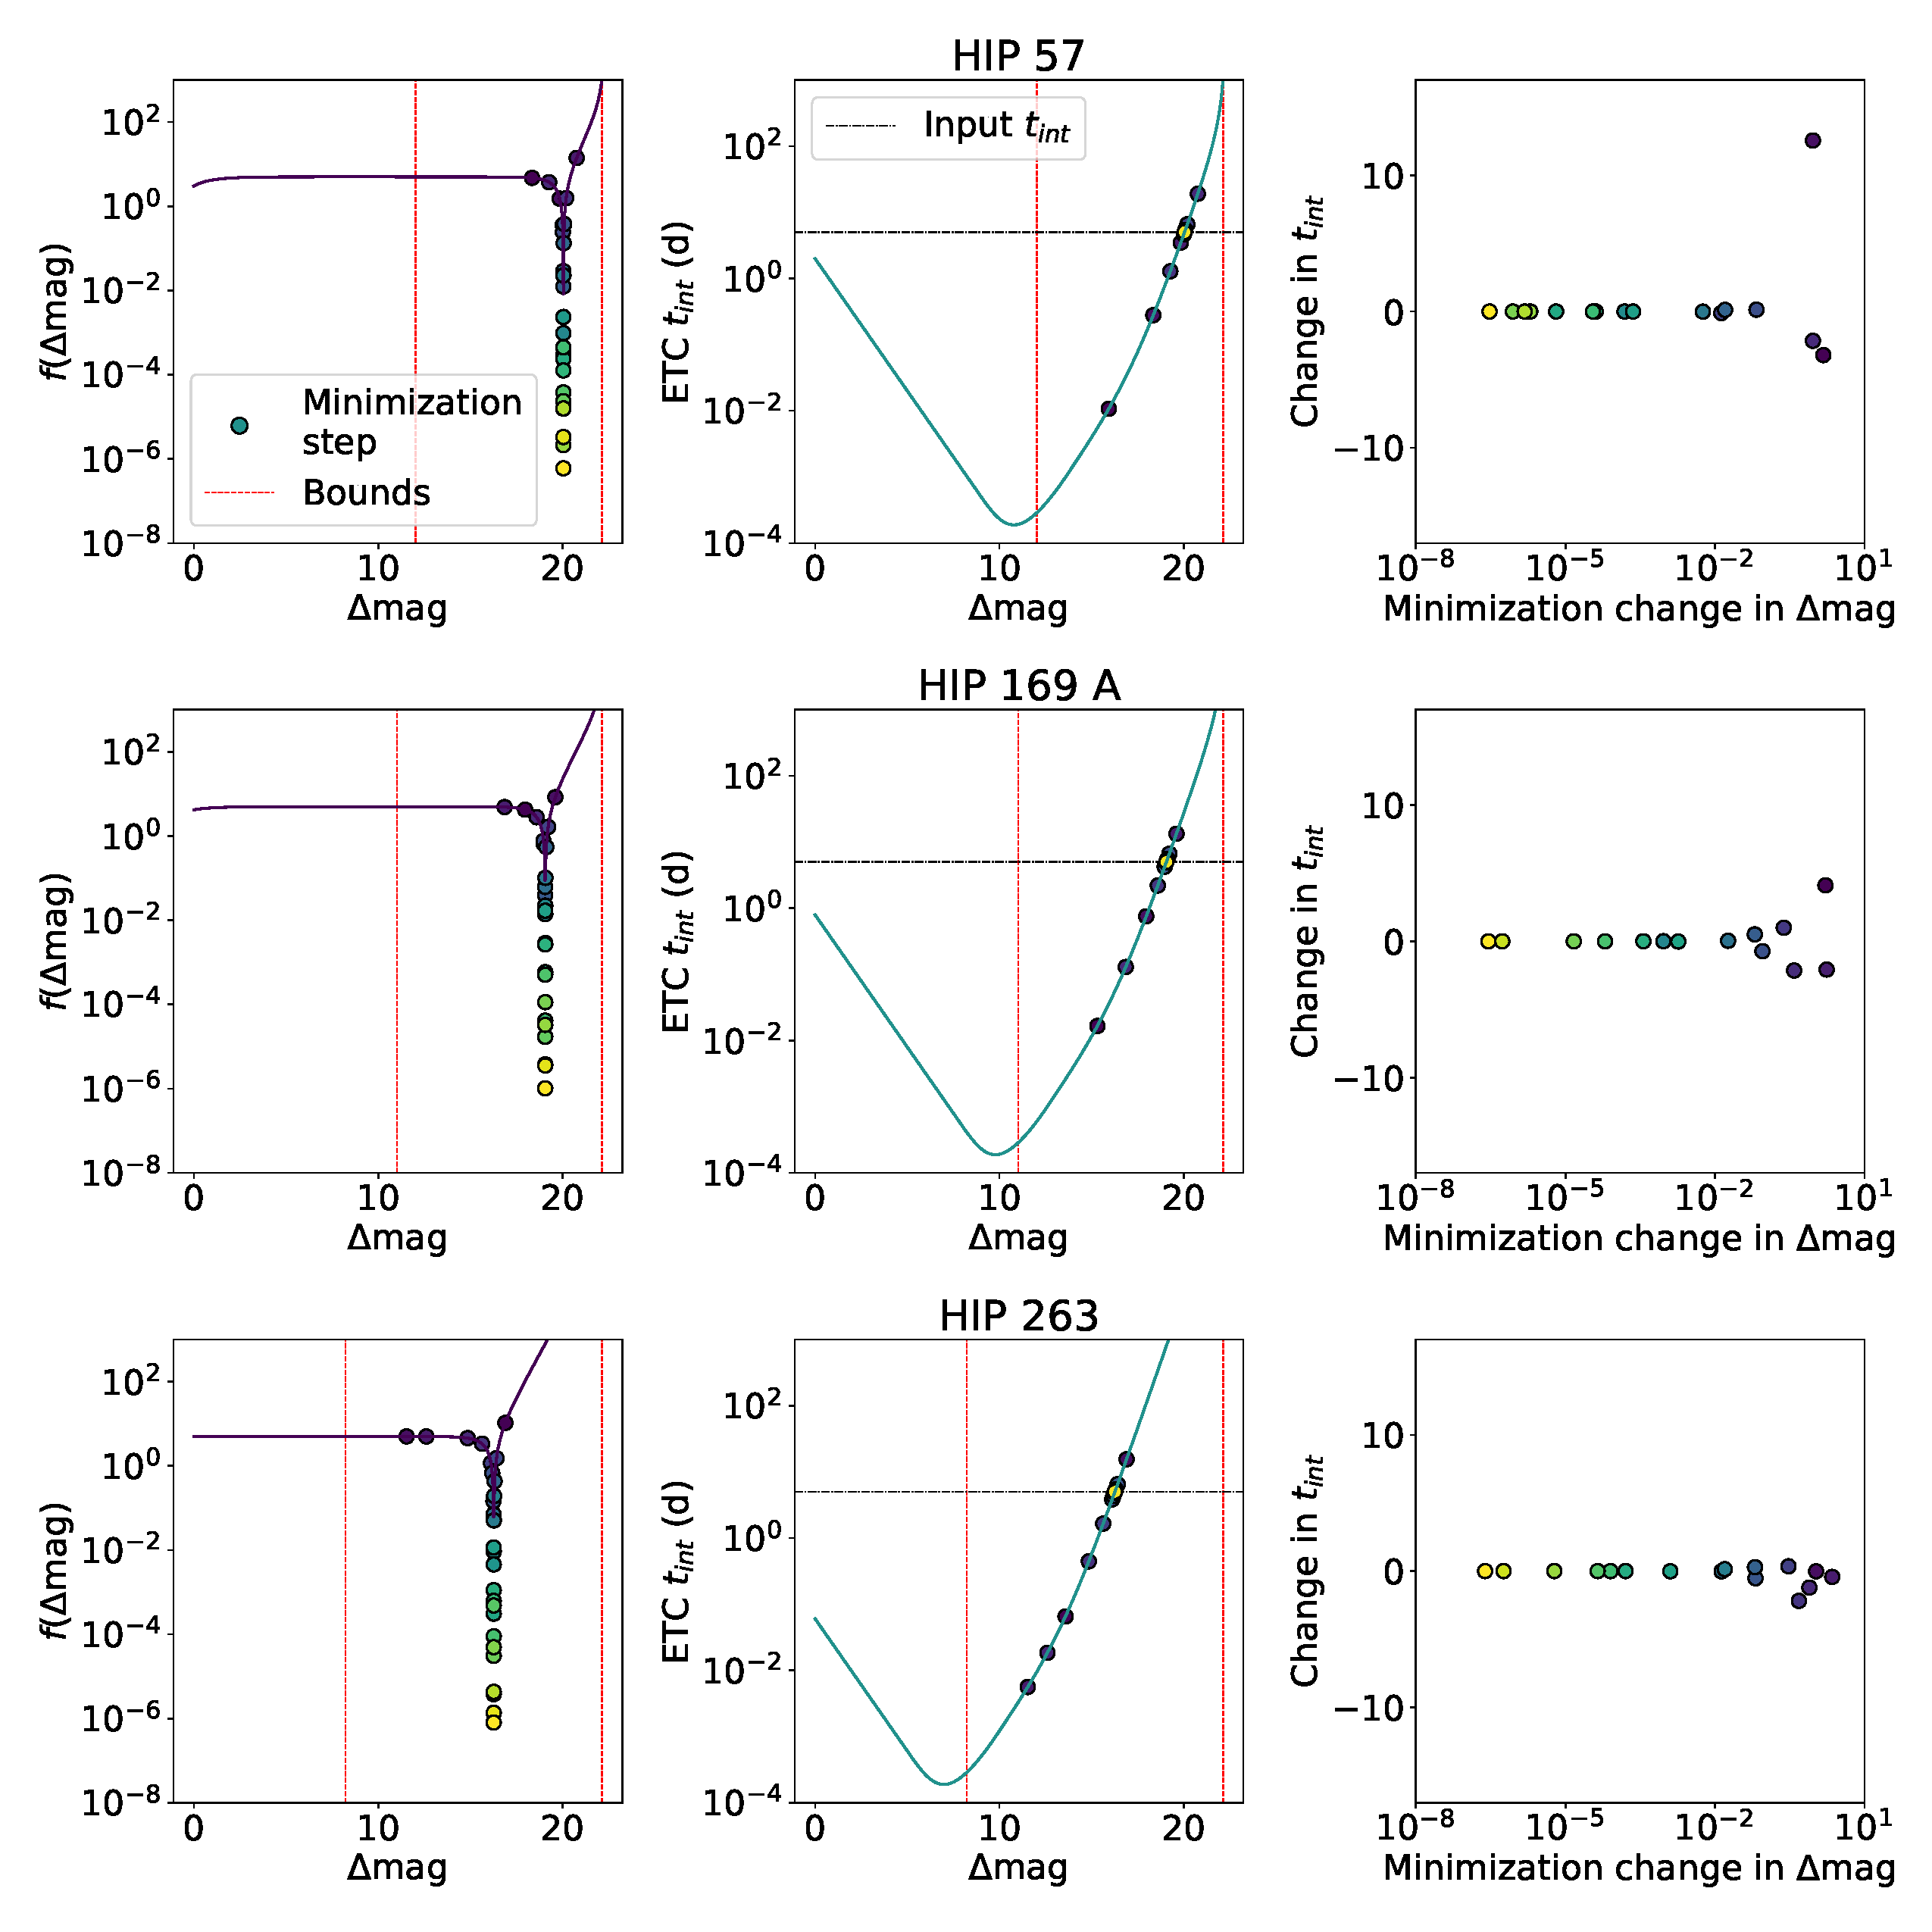
\includegraphics[width=0.95\textwidth]{ch2/figures/minimzation_star_comp.pdf}
  \end{center}
  \caption{Demonstrating successful inversion of the Roman CGI's ETC using the minimization
    routine on HIP 57, HIP 169 A, and HIP 263. Each dot represents a step the
  minimization routine took, with the first step in dark purple and the last in
bright yellow. Each row represents a specific star. The left column shows the
minimization steps compared to the minimization objective function,
\Cref{eq:intTime_root_obj}, and the $\Delta\textrm{mag}$ bounds given to the
minimization routine. The middle column shows the corresponding integration
times for the steps taken by the minimization routine, the $\Delta\textrm{mag}$
bounds, and the input $t_\textrm{int}$ that the minimization routine is
attempting to converge to. The right column shows the $\Delta\textrm{mag}$ step
sizes and their corresponding change in $t_\textrm{int}$.}
  \label{fig:minimization_star_comp}
\end{figure}

\begin{figure}
  \begin{center}
    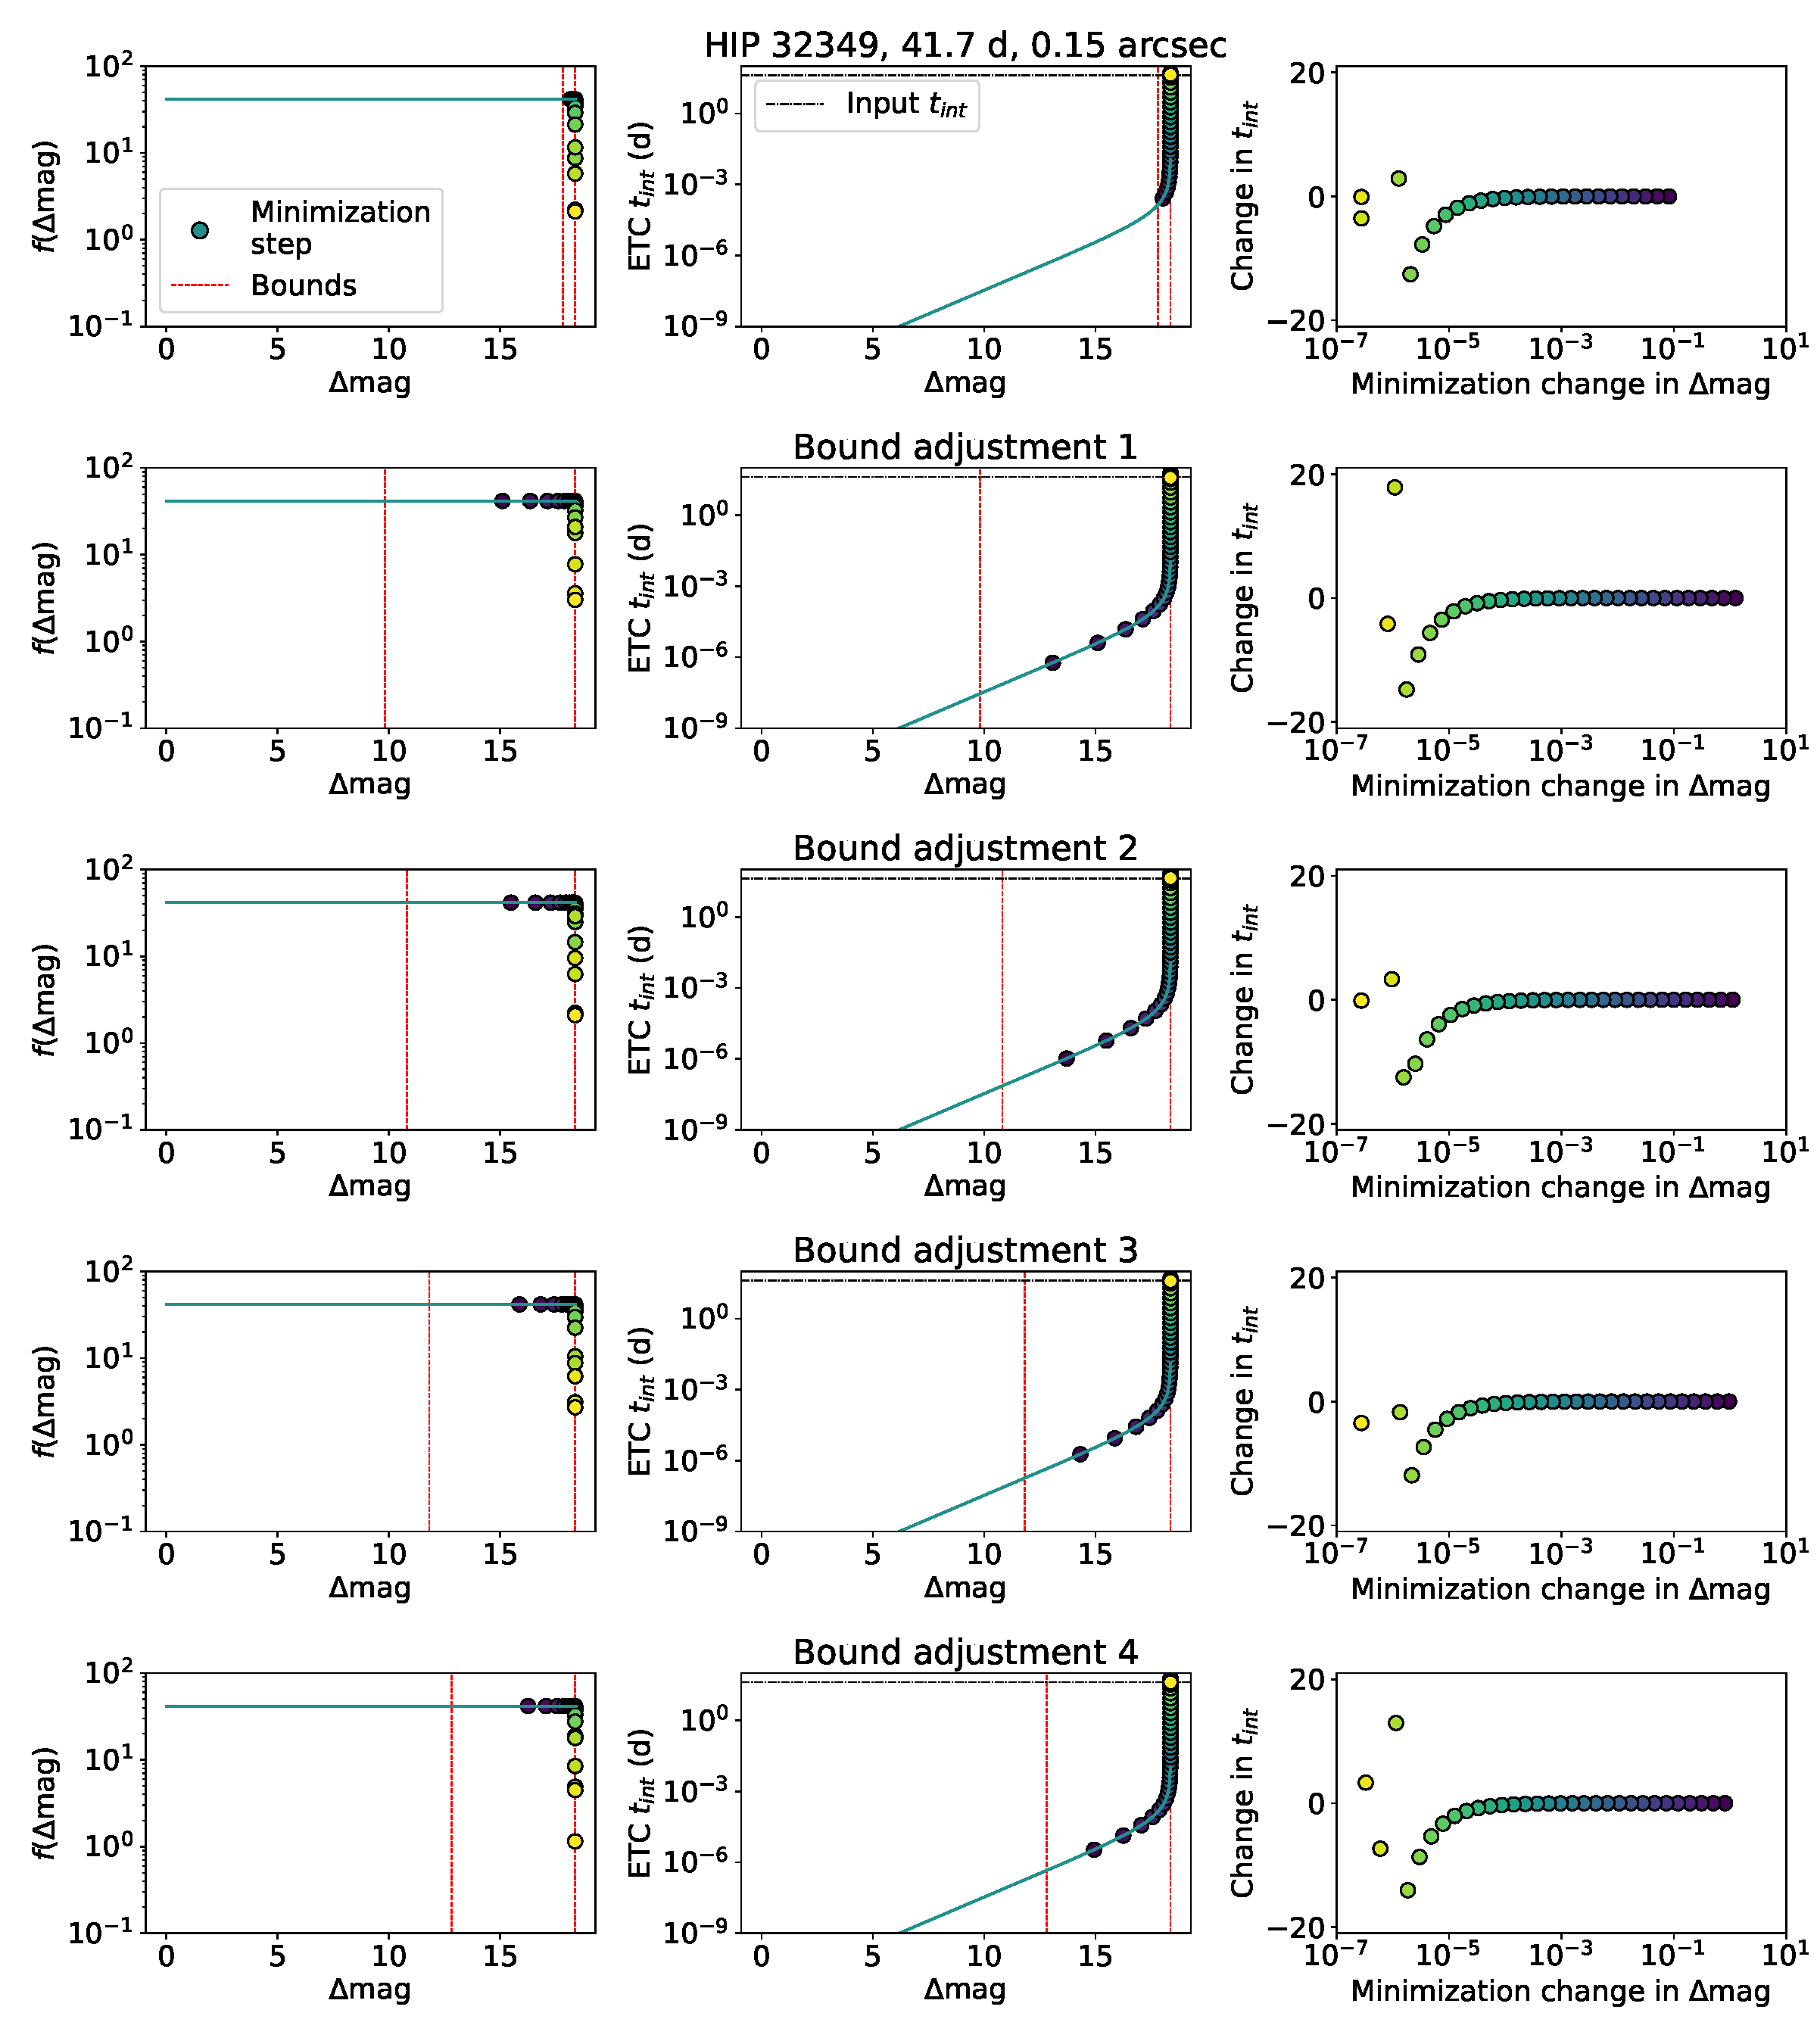
\includegraphics[height=0.75\textheight]{ch2/figures/minimzation_bound_comp.pdf}
  \end{center}
  \caption{The minimization process succeeding with an exceptionally difficult
    scenario, right on the inner working angle of Roman CGI's narrow field
    instrument with a long integration time requested. The progression of the
    lower bounds is shown from top to bottom. The algorithm ultimately finds a
  solution within the 5\% tolerance on the fifth minimization. Note the large
changes in integration time during the last steps which are on the order of
$10^{-6}$ $\Delta\textrm{mag}$.}
  \label{fig:minimzation_bound_comp}
\end{figure}

The two problems we can run into are converging to the lower bound and trying
to find the $\Delta\textrm{mag}$ for an integration time where the greater of the
minima is on the asymptote. In extreme cases the slope of $(\Delta  t_{\textrm{int}}) /
\left(\Delta(\Delta\textrm{mag})\right)$ can be too great for the minimization
routine to converge to the requested tolerance. To handle this we wrap the
minimization in a loop. If the minimization converges to the lower bound, the
lower bound is raised by one and the minimization is run again. If the
resulting lower bound is greater than the upper bound then \Cref{eq:dMag_lb} is
modified to subtract 10 instead of 2. For the case where the solution is on the
asymptote, we allow the routine to stop when the solution value is within 5\% of
the given integration time as the $\Delta\textrm{mag}$ error will be on the
order of $10^{-7}$. \Cref{fig:minimzation_bound_comp} demonstrates the worst
case scenario, where the solution was found after 5 minimization iterations,
found by running the root-finding method on 100 combinations of $t_\textrm{int}$ and
$\alpha$ for all of the stars in the EXOCAT target list
\citep{turnbullExoCat1Nearby2015} with all of the observing scenarios in the
Roman CGI ETC (\url{github.com/hsergi/Roman_Coronagraph_ETC}). If no solution
is found the function will raise an error and exit, indicating that under no
scenario will the exposure time calculator return the inputted integration time.

\begin{figure}
  \begin{center}
    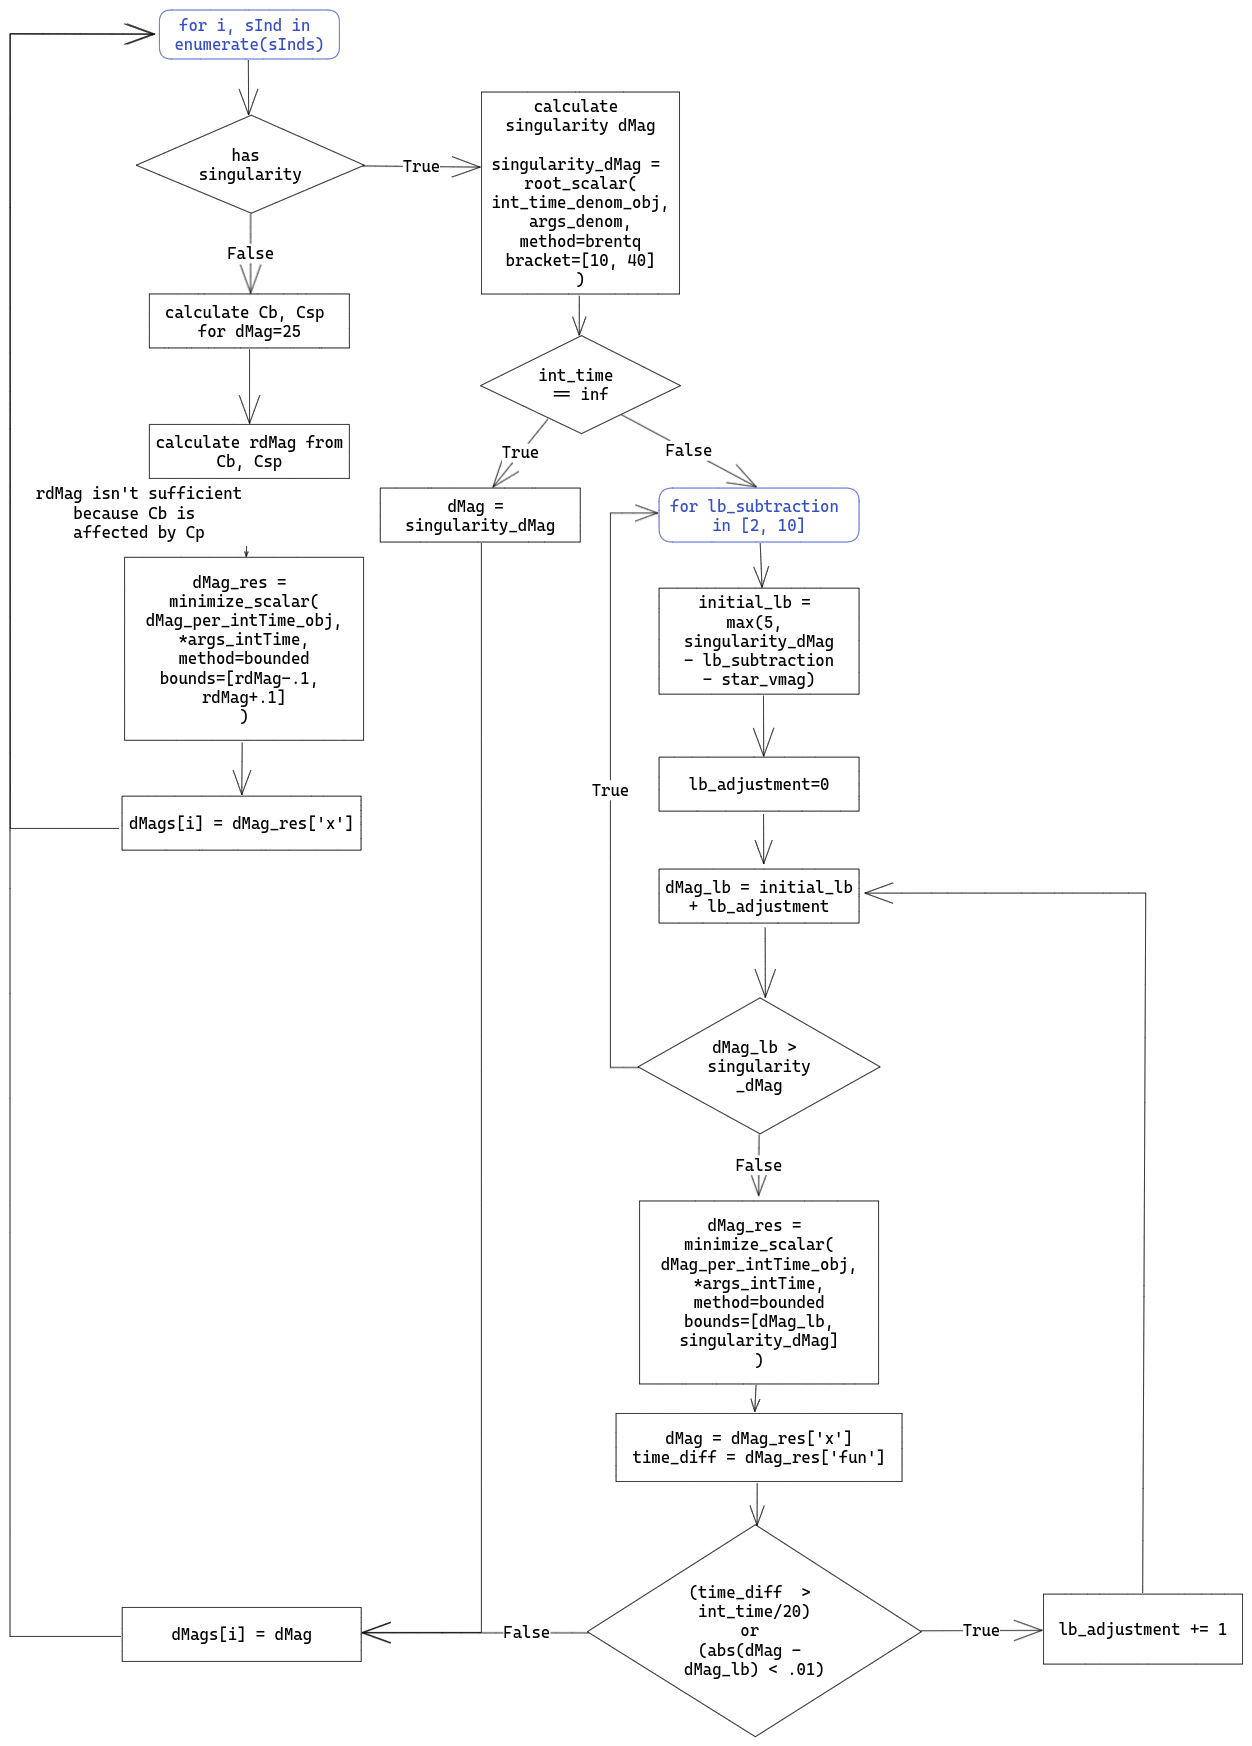
\includegraphics[width=0.95\textwidth]{ch2/figures/root_flowchart.png}
  \end{center}
  \caption{Process of calculating the dimmest detectable $\Delta\textrm{mag}$ given
  an integration time. Uses EXOSIMS naming scheme and Python syntax.}
  \label{fig:root_flowchart}
\end{figure}

The full numerical routine can be seen in \Cref{fig:root_flowchart}.
Effectively the routine turns the flat $\Delta\textrm{mag}_0$ into a function
$\Delta\textrm{mag}_0(t_\textrm{int}, \alpha)$ for the observing scenario of
interest. A major benefit of a numerical routine for solving this is its
robustness. As the optical system models evolve this numerical routine will not
need to be updated in the same fashion that an analytical formulation would.
Additionally, if a change is made to the optical system model and the impact
on an analytical equation for $\Delta\textrm{mag}_0$ is not immediately noticed
it can lead to systematic underestimates or overestimates of the required
observation time to reach a desired completeness.

\section{Results}%
\label{sec:coupling_results}

We worked with the Roman CGI team to establish the completeness of the planets
in NASA Exoplanet Archive \citep{akesonNASAExoplanet2013} for the Roman CGI's
various observing scenarios. The results can be seen in full at the Imaging Mission Database
(\url{plandb.sioslab.com}), a website that pulls all of the planets from the
Exoplanet Archive with sufficient orbital information to establish a density
function of possible $\Delta\textrm{mag}$ and $\alpha$ values as described in
\citet{savranskyExplorationDynamical2019}. The Roman CGI team created eighteen
observing scenarios of interest, three of the four observing modes for three
$t_\textrm{int}$ times each (``minimum'', ``medium'', and ``maximum''), with 2
different error budgets. The observing modes are narrow field imaging, wide
field imaging, and spectroscopy.

The narrow field imaging is achieved with the hybrid Lyot coronagraph with a
filter centered at 575 nm, wide field imaging is done with a shaped pupil
coronagraph (SPC) with a filter centered at 825 nm, and spectroscopy is done
with a separate SPC in a ``bowtie'' shape with a filter centered at 730 nm
\citep{kasdinNancyGrace2020}. 
% For a full description of the observing modes see \citet{kasdinNancyGrace2020},
% but here is a short description of each.
The imaging modes were considered at $t_\textrm{int}$ values of 25, 100, and
10000 hours while the spectroscopy mode was considered at $t_\textrm{int}$
values of 100, 400, and 10000 hours. These times were chosen to represent
short, medium, and infinite integration times. Finally, the observing modes had
both an ``Optimistic'' and ``Conservative'' error budget based on the model
uncertainty factors (MUF) established internally by the Roman CGI team. 
Individual observing scenarios are labeled as a combination of all of these
factors, e.g. ``Conservative NF Imager 25hr''.

\begin{figure}
  \begin{center}
    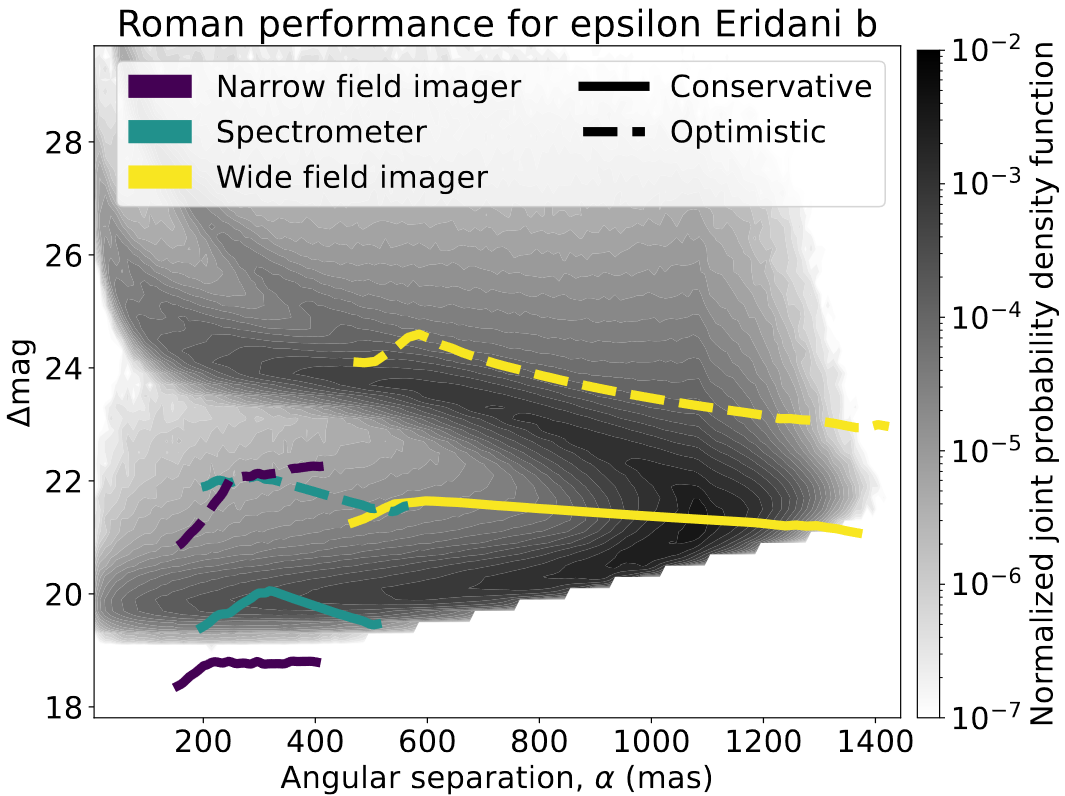
\includegraphics[width=0.95\textwidth]{ch2/figures/RST_performance_flipped.png}
  \end{center}
  \caption{The performance of the Nancy Grace Roman Space Telescope's coronagraph
    instruments when observing the planet epsilon Eridani b. ``Optimistic'' is the
  optimistic error budget with maximum integration time while ``Conservative''
  is the conservative error budget with minimum integration time.}
  \label{fig:RST_performance_flipped}
\end{figure}

For each observing scenario, the $t_\textrm{int}$ value is specified so our
$\Delta\textrm{mag}_0$ is strictly a function of $\alpha$, where $\alpha \in
[\textrm{IWA}, \textrm{OWA}]$ for the observing mode's IWA and OWA. By applying
the method described in \Cref{sec:numerically_inverting_ETC} we generated the
$\Delta\textrm{mag}_{0,i,j}(\alpha)$ values for every star $i$ in the
Imaging Mission Database for the 18 observing scenarios $j$. The joint density
functions $f_k(\Delta\textrm{mag}, \alpha)$ for each planet $k$ were already
calculated for the known planets, as described in
\citet{savranskyExplorationDynamical2019}. We can then calculate the
completeness for a planet $k$ around star $i$ with observing scenario $j$
\begin{equation}
  c_{j,k} = \int_{\textrm{IWA}_j}^{\textrm{OWA}_j}\int_0^{\Delta\textrm{mag}_{0,i,j}(\alpha)} 
  f_k (\Delta\textrm{mag}, \alpha)
  \textrm{d}\Delta\textrm{mag}\textrm{d}\alpha
  \label{eq:c_plandb}
\end{equation}
which allows us to estimate the sensitivity of the various observing scenarios
to known planets. This can be visualized by overlaying the
$\Delta\textrm{mag}_{0,i,j}(\alpha)$ lines on a joint density function
$f_k(\Delta\textrm{mag}, \alpha)$, as shown in
\Cref{fig:RST_performance_flipped}, and looking at the area under a given
$\Delta\textrm{mag}_{0,i,j}(\alpha)$ line. The completeness values for the
scenarios in \Cref{fig:RST_performance_flipped} are shown in
\Cref{tab:eps_eri_table}, demonstrating that wide field imaging mode has the highest
completeness for epsilon Eridani b. \Cref{tab:eps_eri_table} shows that for the narrow field
imager, increasing $t_\textrm{int}$ has almost no effect because the narrow field imager is effectively
at the saturation point at $t_\textrm{int}=25$ for epsilon Eridani. The wild field
imager is not at the saturation point at $t_\textrm{int}=25$ which results in a
difference of $\sim$0.077 $c$ between $t_\textrm{int}=25$ hr and
$t_\textrm{int}=100$ hr.

\begin{table}
  \caption{Completeness of epsilon Eridani b under the 18 different observing scenarios.}
  \label{tab:eps_eri_table}
  \begin{center}
    \begin{tabular}{|cccc|}\hline
      \bfseries Scenario &
      \bfseries Minimum $t_\textrm{int}$ &
      \bfseries Medium $t_\textrm{int}$ &
      \bfseries Maximum $t_\textrm{int}$
      \csvreader[head to column names]{ch2/figures/eps_eri.csv}{}
      {\\\hline\csvcoli\ & \csvcolii & \csvcoliii & \csvcoliv}
      \\\hline
    \end{tabular}
  \end{center}
\end{table}

This process was run on all planets in the Exoplanet Archive and the resulting
completeness values were incorporated into the Imaging Mission Database. The
ten highest completeness planets and the observing scenarios to maximize
completeness for the planets are shown in
\Cref{tab:top_comp_planets}.
\begin{table}
  \caption{Highest completeness planets on \url{plandb.sioslab.com} and their respective
  observing mode.}
  \label{tab:top_comp_planets}
  \begin{center}
    \begin{tabular}{|c|c|c|c|}\hline
      \bfseries Planet &\bfseries $c$ &\bfseries Observing scenario
      \csvreader[head to column names]{ch2/figures/plandb_data.csv}{}
      {\\\hline\csvcoli\ & \csvcolii & \csvcoliii}
      \\\hline
    \end{tabular}
  \end{center}
\end{table}

\section{Conclusion}

In this chapter, we have demonstrated that the current exposure time calculator
for the Roman Space Telescope's coronagraph instrument cannot be analytically inverted to
isolate $\Delta\textrm{mag}$ as a function of $t_\textrm{int}$ because the
background signal is a function of the $\Delta\textrm{mag}$ value. We have
demonstrated how to handle completeness calculations with that limitation by
inverting the ETC with a numerical minimization routine implemented in
\code{EXOSIMS}. With this routine, we can establish the photometric constraint
($\Delta\textrm{mag}_0$) for the calculation of completeness for any observing
scenario when there is a coupling between the planet and background signals. By
calculating the $\Delta\textrm{mag}_0$ value over a range of $\alpha$ values we
can account for the change in throughput at smaller separations and avoid
systematically overestimating the completeness values for planets at small
separations. We applied this process to create the Roman Space Telescope's
observing scenario completeness values for the Imaging Mission Database. By
using the Imaging Mission Database a researcher can see the sensitivity of the
various Roman CGI observing modes to different known planets.

% sec:Coupling of background and planet signal (end)

% This dependence is somewhat hidden, but it begins with equation 48 of \citet{Nemati2020a},
% \begin{equation}
%   \sigma_{\textrm{det}}^2 = i_d m_{\textrm{pix}} t + q_\textrm{CIC} m_{\textrm{pix}} \frac{t}{t_{\textrm{fr}}}
%   + m_{\textrm{pix}} \frac{t}{t_{\textrm{fr}}} \left( \frac{\sigma_{\textrm{rd}}}{G_{\textrm{EM}}}\right)^2
%  \label{eq:bijan_detector_noise}
% \end{equation}
% where $\sigma_{\textrm{det}}^2$ is the CCD detector noise variance, $i_d$ is
% the detector dark current, $m_{\textrm{pix}}$ is the number of detector pixels
% that the planet signal covers, $t_\textrm{int}$ is the integration time, $q_{\textrm{CIC}}$
% is the CCD clock-induced charge, $t_{\textrm{fr}}$ is the frame duration,
% $\sigma_{\textrm{rd}}$ is read noise, and $G_{\textrm{EM}}$ is the electron
% multiplication gain. $\sigma_{\textrm{det}}^2$ is one of the four random
% noise components for the target star in $C_{\textrm{b},i}$, see \citet{Nemati2020a} for more details.
% The $t_\textrm{int}/t_{\textrm{fr}}$ terms in equation~\ref{eq:bijan_detector_noise} are
% equal to the number of frames collected over the full integration time $t_\textrm{int}$,
% which is where the coupling between the planet and noise ultimately comes from.
% The way that the frame time calculation has been implemented in the Roman ETC
% is
% \begin{equation}
%   t_{\textrm{fr}} = \frac{0.1}{DC +\left(r_{\textrm{pl,ia}}+r_{\textrm{zo,ia}}+r_{\textrm{sp,ia}}\right)/m_{\textrm{pix}}}
%   \label{eq:bijan_frame_duration}
% \end{equation}
% where $DC$ is the detector dark current noise per second, $r_{\textrm{pl,ia}}$ is
% the planet electron count rate at the image area per pixel per second,
% $r_{\textrm{zo,ia}}$ is the zodiacal light electron count rate at the image area
% per pixel per second, $r_{\textrm{sp,ia}}$ is the speckle electron count rate at
% the image area per pixel per second, and is cut to be between 1 and 80 seconds. This
% is not in literature and was pulled from a private GitHub repository that hosts the
% ETC.

% The equation for $r_{\textrm{pl,ia}}$ is
% \begin{equation}
%   r_{\textrm{pl,ia}} = F_p f_{\textrm{SR}} A_{\textrm{col}} \textrm{QE} \tau_{\textrm{PS}}
%   \label{eq:bijan_planet_ia}
% \end{equation}
% where $F_p$ is the planet's flux, $f_{\textrm{SR}}$ is the fraction of light in
% the signal region, $A_{\textrm{col}}$ is the collecting area of the primary, QE
% is the quantum efficiency, and $\tau_{\textrm{PS}}$ is the throughput of a
% point source. By expressing the planet's flux in terms of the star's flux $F_s$
% and $\Delta\textrm{mag}$,
% \begin{equation}
%   F_p = F_s 10^{-\Delta\textrm{mag}/2.5},
%   \label{eq:fp_dmag}
% \end{equation}
% we see how the $\Delta\textrm{mag}$ term ends up in the calculation of
% $C_{\textrm{b}}$. If the $r_{\textrm{pl,ia}}$ term was removed from
% equation~\ref{eq:bijan_planet_ia} the coupling would be removed, but it is
% prudent to account for the planet's signal, especially for observing scenarios
% which consider bright planets.

% To complicate the relationship further, the $t_{\textrm{fr}}$ value impacts the
% number of cosmic ray hits per frame and the charge transfer efficiency. Those
% end up impacting the detector degradation (dQE) which then impacts the count
% rates for the planet, zodiacal light, and extra zodiacal light. This makes it
% impossible to invert the exposure time calculator and isolate
% $\Delta\textrm{mag}$ as a function of integration time analytically. Our approach,
% laid out in Section~\ref{sec:numerically_inverting_ETC} explains our numerical
% solution with root finding.

% Figure~\ref{fig:CGI_coupling} shows the errors that occur when trying to
% calculate the $\Delta\textrm{mag}_0$ values with equation~\ref{eq:dean_dmag},
% the colored circles. The true $\Delta\textrm{mag}$ values, the empty circles,
% deviate significantly and in many cases would result in underestimating
% $\Delta\textrm{mag}_0$. The direction of the error is driven by how close the
% $\Delta\textrm{mag}_0$ is to the saturation $\Delta\textrm{mag}$, or the
% $\Delta\textrm{mag}$ at which $\left(\textrm{SNR} \cdot C_{\textrm{sp}}\right)^2$ becomes greater than $C_{\textrm{p}}$ in
% equation~\ref{eq:dean_inttime} and the calculated integration times become
% negative.

% Further, the impact on completeness is incredibly difficult to characterize,
% since that the zodiacal light terms are involved.

% Figure~\ref{fig:dMag_error} shows the problem of trying to calculate
% $\Delta\textrm{mag}$ without accounting for the coupling. The ``Assumed $\Delta
% \textrm{mag}$'' refers to the user-inputted $\Delta \textrm{mag}$ that is used
% when calculating $C_{\textrm{b}, i}$. The highest assumed $\Delta \textrm{mag}$
% of 15 shows the worst performance, while the lowest assumed $\Delta
% \textrm{mag}$ of 25 has relatively small errors. This coupling is significant
% in many cases, and makes it impossible to analytically solve for
% $\Delta\textrm{mag}$ as a function of integration time. Therefore we must
% approach it as a numerical problem.
